\documentclass[10pt, a4paper]{article}
\usepackage[english]{babel}

% matlab code
\usepackage[numbered,framed]{matlab-prettifier}
\let\ph\mlplaceholder % shorter macro
\lstMakeShortInline"
\lstset{
  style              = Matlab-editor,
  basicstyle         = \mlttfamily,
  escapechar         = ",
  mlshowsectionrules = true,
  breaklines=true,
}
\usepackage{adjustbox}

% For subfigure use
\usepackage[font=small,labelfont=bf]{caption}
\usepackage{subcaption}

% Set page size and margins
% Replace `letterpaper' with`a4paper' for UK/EU standard size
\usepackage[a4paper,top=2cm,bottom=2cm,left=2cm,right=2cm,marginparwidth=2cm]{geometry}

% tabelas
\usepackage{array}
\usepackage{tabularx}
\usepackage{booktabs}

\usepackage{float}

% Useful packages
\usepackage{amsmath}
\usepackage{graphicx}
\graphicspath{{figures/}} %Setting the graphicspath
\usepackage[colorlinks=true, allcolors=blue]{hyperref}

\title{System Identification 07 - Grey box models \\ \large Professor: Helon Vicente Hultmann Ayala}

\author{Felipe da Costa Pereira \\ {\tt felipecostapereira@gmail.com}}
\begin{document}

\maketitle


\section{Activity}

\begin{itemize}
      \item
      Rodar o c{\'o}digo de identifica{\c c}{\~a}o do EMPS fornecido e analisar linha por linha o funcionamento.
      \item
      Trocar o modelo de Coulomb pelo modelo de Tustin (eq 10 do artigo abaixo): \\
      \url{https://www.sba.org.br/open_journal_systems/index.php/cba/article/view/1570} \\
      Comparar os resultados: Coulomb vs. Tustin (em termos de erro, par{\^a}metros identificados, etc)
      \item
      Caso tenham interesse em se aprofundar nos modelos de atrito, podem testar com demais op{\c c}{\~o}es no artigo de revis{\~a}o abaixo: \\
      \url{https://link.springer.com/content/pdf/10.1007/s11071-016-2999-3.pdf} \\
      Sugiro tentar o Lugre (secao 3.5 deste artigo) - atividade extra (para os interessados).
\end{itemize}

\section{Code Changes}

In order to use the Tustin model for the friction force as proposed, the torque expression changes from equation \ref{eq:1} to equation \ref{eq:2} described below:     \newline


Torque expression using Coulomb friction force model:
\begin{equation}\label{eq:1}
      \tau(t) = M\ddot{q}(t) + F_{v}\dot{q}(t) + F_{c}sign(\dot{q}(t)) + offset
\end{equation}

Torque expression using Tustin friction force model:
\begin{equation}\label{eq:2}
      \tau(t) = M\ddot{q}(t) + F_{v}\dot{q}(t) + F_{c}sign(\dot{q}(t)) + (F_{s} - F_{c})e^{-\frac{|\dot{q}|}{v_{s}}} + offset
\end{equation}


Parameters and $\dot{x_{2}}=\ddot{q}$ expresion on the state vector: \\ \\
\begin{adjustbox}{max width=\textwidth}
      \begin{lstlisting}
            Mn    = MX.sym('Mn');
            Fvn   = MX.sym('Fvn');
            Fcn   = MX.sym('Fcn');
            Fsn   = MX.sym('Fsn');
            vsn   = MX.sym('vsn');
            ofstn = MX.sym('ofstn');

            params   = [Mn;Fvn;Fcn;Fsn;vsn;ofstn];
            parammax = [150; 300; 40; 40; 1e-3; 15];
            parammin = [ 30; 100;  0;  0; 1e-4; -15];

            % rhs = [dq; (u-Fv*dq-Fc*sign(dq)-ofst)/M];
            rhs = [dq;(u-Fv*dq-Fc*sign(dq)+(Fc-Fs)*exp(-(abs(dq))/vs)-ofst)/M];
      \end{lstlisting}
\end{adjustbox} \\

The range for the $v_{s}$ parameter was based on the respecitve value given by the IDIM model ($v_{s} = 0.006464$). The rest of the code is kept exactly the same.

\newpage

\section{Results}

After performing the grey box identification using the casadi library, we compare the parameters values estimated by the inverse dynamic model (IDM) and the grey box casadi model. The values of the estiamted parameters, for both the Coulomb and the Tustin friction forces are shown in tables \ref{table:m1} and \ref{table:m2}.

\begin{table}[H]
      \small
      \centering
      \caption{Coulomb Model parameters}
      \begin{tabular}{c|c|c|c|c}
            Model &  M & Fv & Fc & ofst \\
            \hline
            casadi & 95.1089 & 203.5034 & 20.3935 & -3.1648 \\
            IDIM   & 96.0014 & 213.8943 & 19.4167 & -3.2790 \\
      \end{tabular}
      \label{table:m1}
\end{table}

\begin{table}[H]
      \small
      \centering
      \caption{Tustin Model parameters}
      \begin{tabular}{c|c|c|c|c|c|c}
            Model &  M & Fv & Fc & Fs & vs & ofst \\
            \hline
            casadi & 97.001 & 222.01 & 18.606 & 36.3311 & 0.000900 & -3.29 \\
            IDIM   & 95.681 & 203.36 & 17.023 & 17.0230 & 0.006464 & -4.12 \\
      \end{tabular}
      \label{table:m2}
\end{table}

The simulated responses and the associeted errors, for both force models (Coulomb and Tustin) and parameters estimation methods (casadi amd IDIM) are show in figures \ref{fig:y} and \ref{fig:e}.

As we can notice, casadi models estimate have a good fit for both force models, while IDIM models have a poor performace (higher error) when estimating the Tustin force model parameters.

\begin{figure}[H]
      \centering
      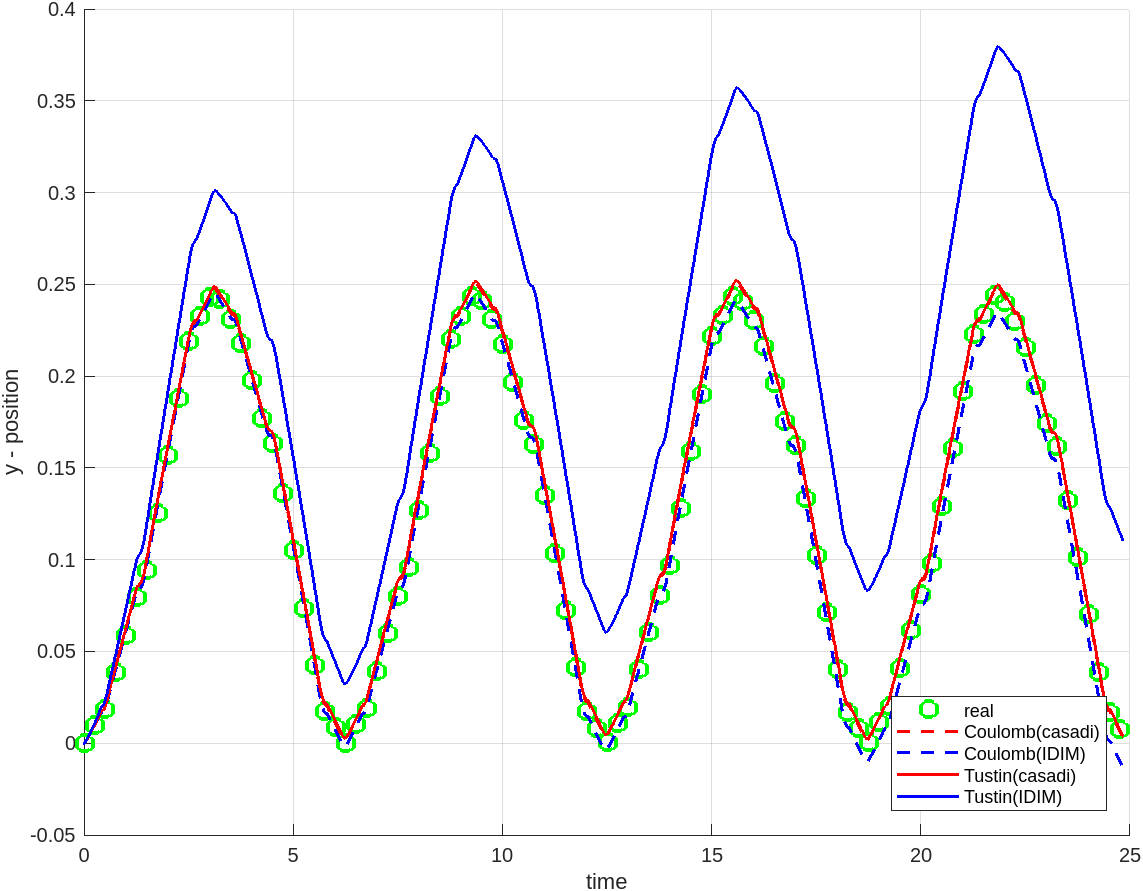
\includegraphics[width=0.8\textwidth]{y.PNG}
      \caption{Position (y) - real and estimated data}
      \label{fig:y}
\end{figure}

\begin{figure}[H]
      \centering
      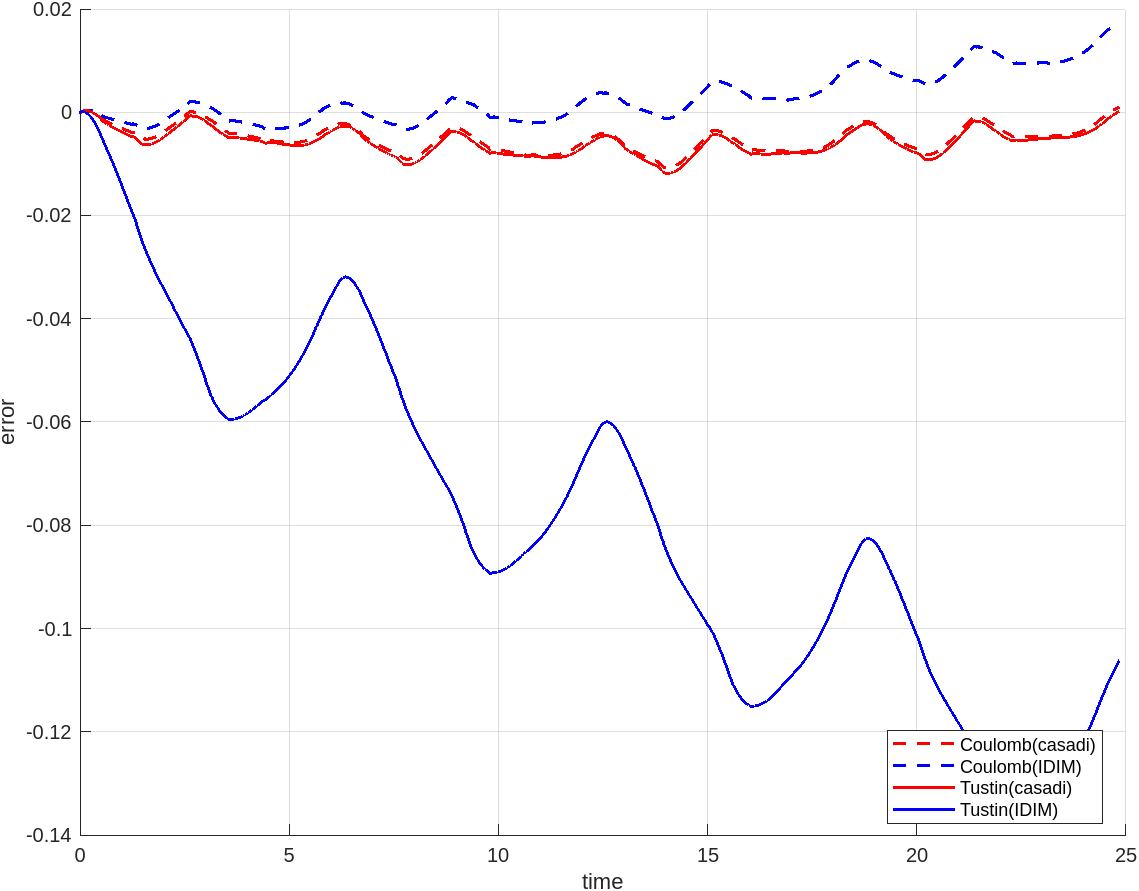
\includegraphics[width=0.8\textwidth]{e.PNG}
      \caption{Error between estimated and real data}
      \label{fig:e}
\end{figure}

\end{document}
